\chapter{Design}
\label{design}
This Chapter outlines the overall design of the PARSE toolkit and the design choices made by the group. Each aspect of the system has required prototyping in order to evaluate the best approach to overall integration of the system and so that the requirements in the specification can be met. A high level system overview is presented along with detailed design discussions of each functional part of the system. These include reference to key algorithms, operations and run-time analysis where appropriate. The design section concludes with a consideration of the interface design of the system.

\section{System Implementation}

The implementation of the system describes each component as it was implemented in the final system. In this section, the broad functionality of each component is described. Further subsections discuss the overall accuracy and results achieved from the components implemented. \\

\subsection{CoreLoader}

The main Coreloader screen contains all functionality associated with the system. There are options present for selecting particular Kinect feeds, calibrating the Kinect's position and viewing the debug console. Recent patients are also displayed persistently for quick access to the scans and results of previous scans on a particular patient. Configuration options are also possible through Coreloader such as setting the working directory for PARSE files and attributing .PARSE and .PCD scan files to patients. Exporting scans to .PCD is also here so that scans produced by the System can be visualised using the Point Cloud Library toolkit\footnote{Point Cloud Library, http://www.pointclouds.org}. \\

\begin{center}
    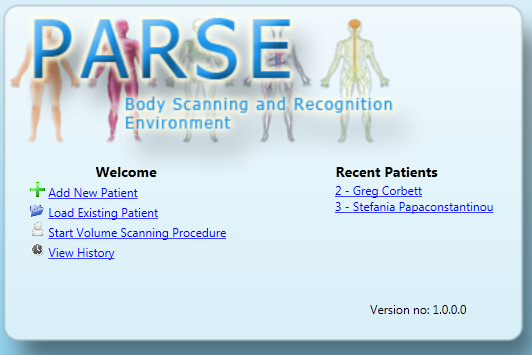
\includegraphics[scale=0.5]{zscreenshots/corewelcome.png}\\
    \caption{CoreLoader welcome screen with toolkit options}
\end{center} \\

\begin{center}
    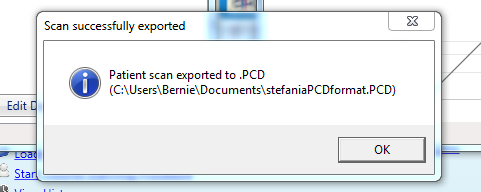
\includegraphics[scale=0.6]{zscreenshots/savetopcd.PNG}\\
    \caption{Confirmation of point cloud file exported to .PCD}
\end{center} \\

\begin{center}
    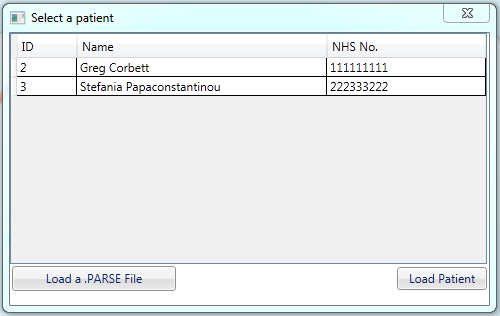
\includegraphics[scale=0.55]{zscreenshots/metaloader.PNG}\\
    \caption{List of patients in the database with associated point cloud or scan information}
\end{center} \\

\begin{center}
    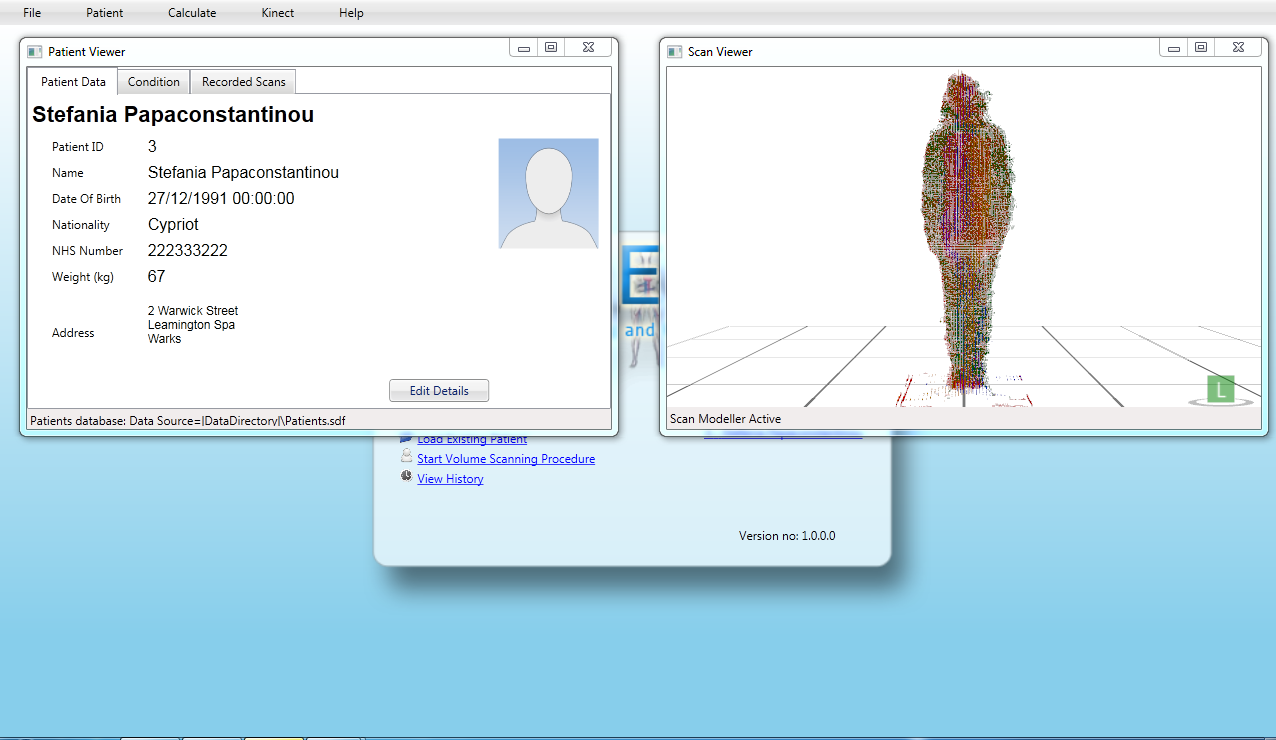
\includegraphics[scale=0.3]{zscreenshots/coreloaderstef.PNG}\\
    \caption{System with scan and associated patient detail displayed}
\end{center} \\


\subsection{ViewLoader}

\begin{center}
    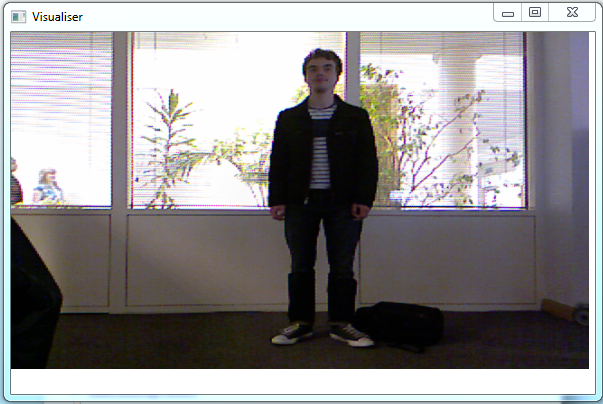
\includegraphics[scale=0.5]{zscreenshots/rgbvisualiser.PNG} \\
    \caption{ViewLoader: Showing the raw RGB feed}
\end{center} \\

Viewloader is capable of displaying raw streams from the Kinect or composite streams that combine multiple views such as depth isolation, colour isolation, or the overlay of a skeleton onto existing feeds. The above image shows the conventional RGB feed from the Kinect. \\

\subsection{ScanLoader}

\begin{center}
    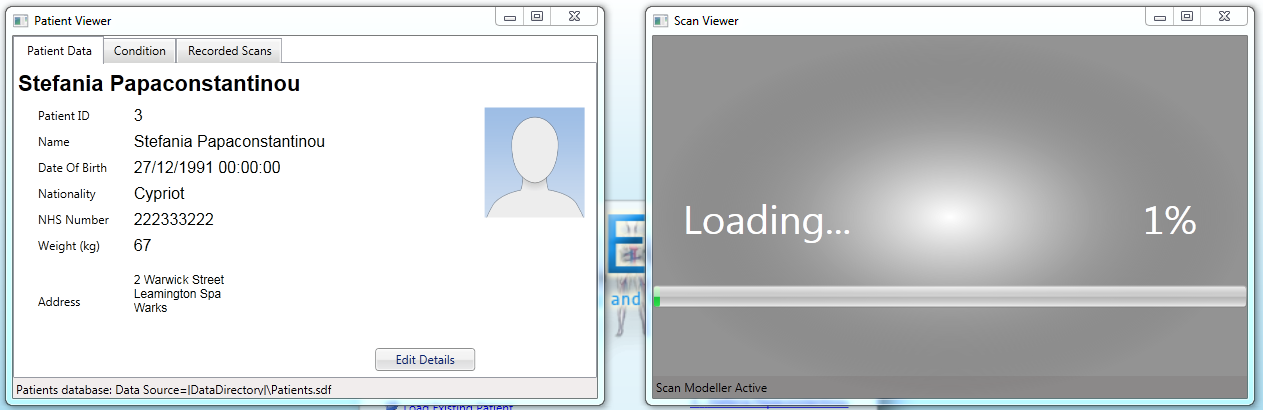
\includegraphics[scale=0.3]{zscreenshots/patientloading.png} \\
    \caption{ScanLoader: The patient data portal (left) and the model viewer loading (right)}
\end{center} \\

\begin{center}
    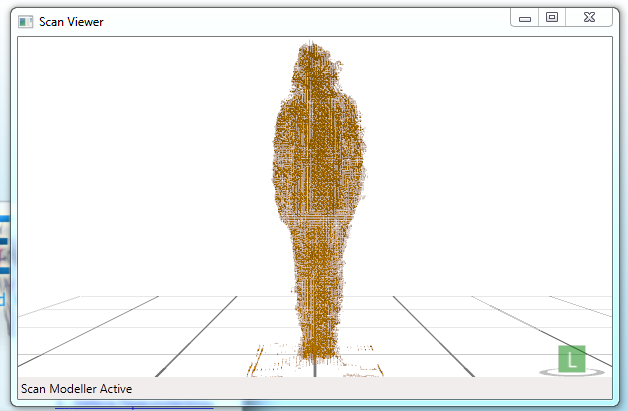
\includegraphics[scale=0.5]{zscreenshots/scanframework.png} \\
    \caption{ScanLoader: 3D model viewport}
\end{center} \\

ScanLoader visualises the registered point clouds from the scan process and allows the model to be viewed from a number of different perspectives and zoom levels. The point cloud visualisation process is resource intensive as approximately 200,000 points are drawn in 3D space. As a result of this, a persistent loading dialog is displayed when the point cloud is being loaded into scan loader or when refining operations are applied to the point cloud. \\

\subsection{HistoryLoader}

\begin{center}
    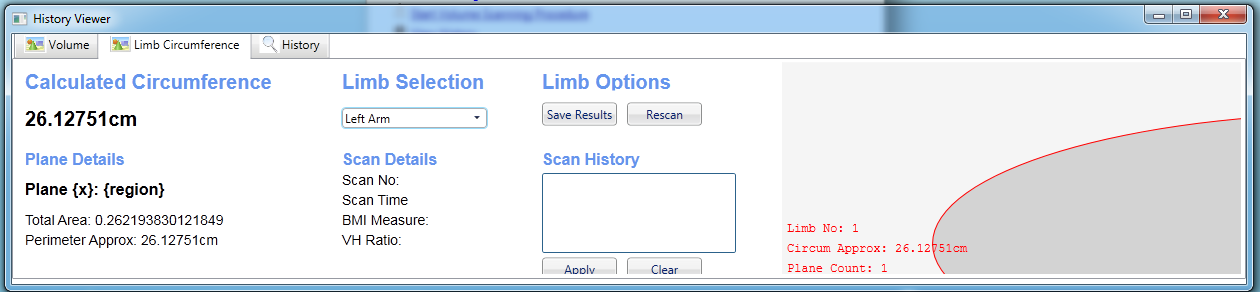
\includegraphics[scale=0.4]{zscreenshots/circumdetail.png}
    \caption{HistoryLoader: Circumference history}
\end{center} \\

\begin{center}
    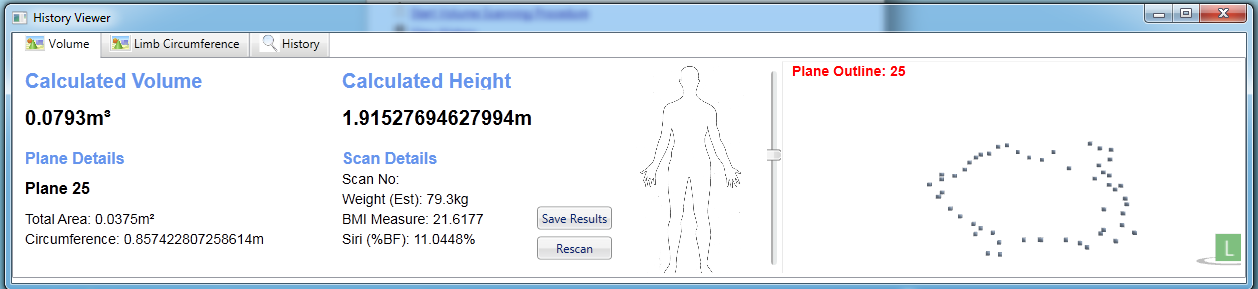
\includegraphics[scale=0.4]{zscreenshots/voldetail.png}
    \caption{HistoryLoader: Volume, height \& plane history}
\end{center} \\

\begin{center}
    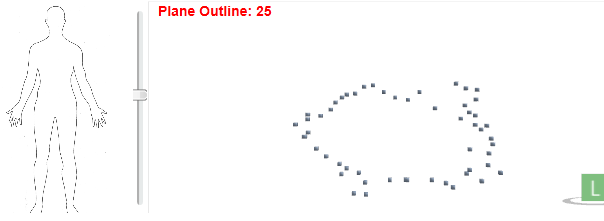
\includegraphics[scale=0.75]{zscreenshots/volumevisualisation.png}
    \caption{HistoryLoader: Plane viewer}
\end{center} \\

The HistoryLoader component of the system visualises the volume and circumference calculation results along with visualisations related to the extrcted planes from the point cloud as well as the visualisation for the approximation of the circumference of the limbs. In each component, different metrics can be visualised for volume in terms of the different planes of the body as well as the circumference for each limb that has been partitioned. These results can then be saved or refined during a rescan procedure. \\

\subsection{PatientLoader}

\begin{center}
    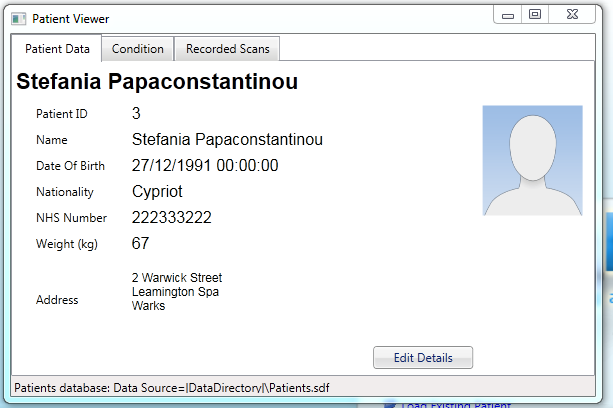
\includegraphics[scale=0.5]{zscreenshots/patientdetail.png} \\
    \caption{PatientLoader: Patient information pane}
\end{center} \\

The PatientLoader presents the patient detail recovered from the database when a patient's scans for either volume/limb circumference or markerless recognition purposes is loaded. PatientLoader also provides the ability to apply new markerless measurements and recover old measurements. Patient information such as personal details and patient conditions can also be added here. \\

\subsection{MeasurementLoader}
MeasurementLoader presents the mechanism for adding a new body-relative scan position with a hand-held sensor. Clear instructions are displayed, indicating to the users how to progress.\\

\begin{enumerate}
    \item Wait for two people to be in view
    \item Search for the sensor device
    \item Use the sensor's location, in combination with the skeletal data, to identify the doctor and the patient
    \item When the sensor is held still for 10 seconds, the system automatically runs the capture routine.
\end{enumerate} \\

\begin{center}
    \setlength\fboxsep{0pt}
    \setlength\fboxrule{0.5pt}
    \fbox{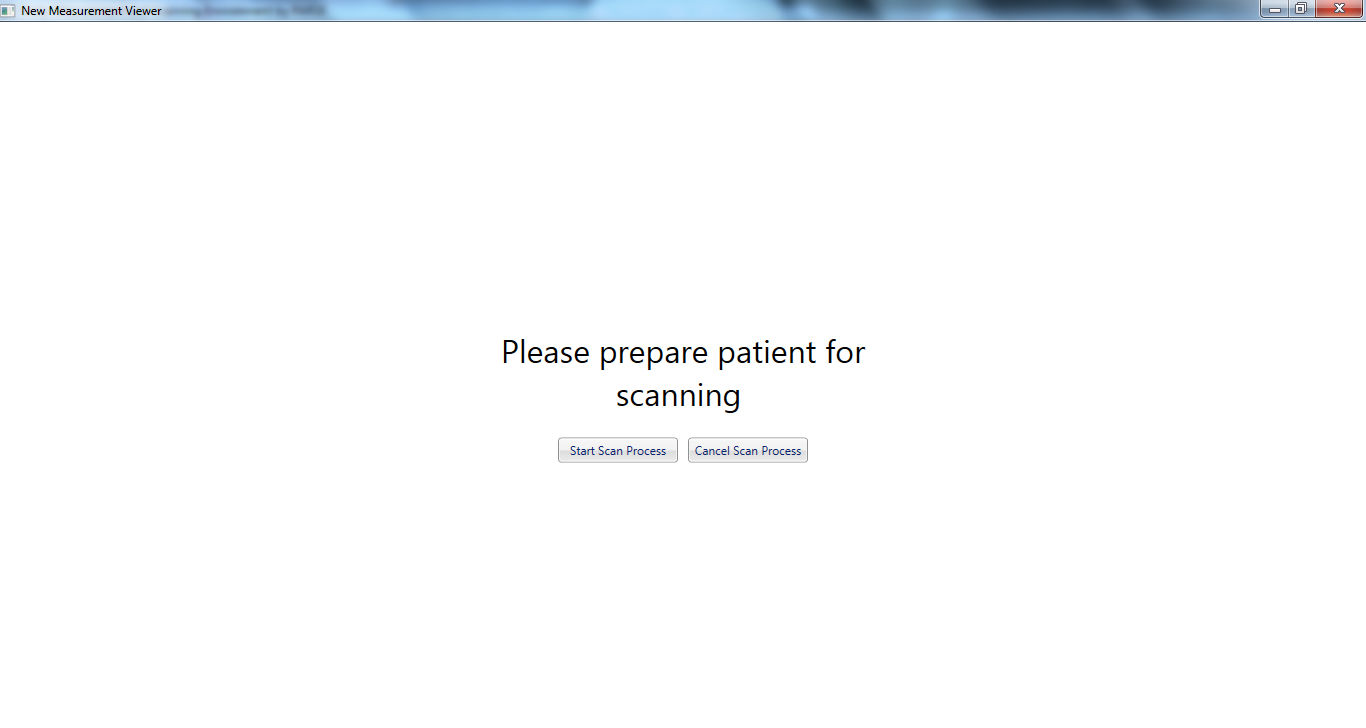
\includegraphics[scale=0.25]{zscreenshots/MeasurementLoader.png}}\\
    \caption{MeasurementLoader: Ready to start a scan}
\end{center} \\

\begin{center}
    \setlength\fboxsep{0pt}
    \setlength\fboxrule{0.5pt}
    \fbox{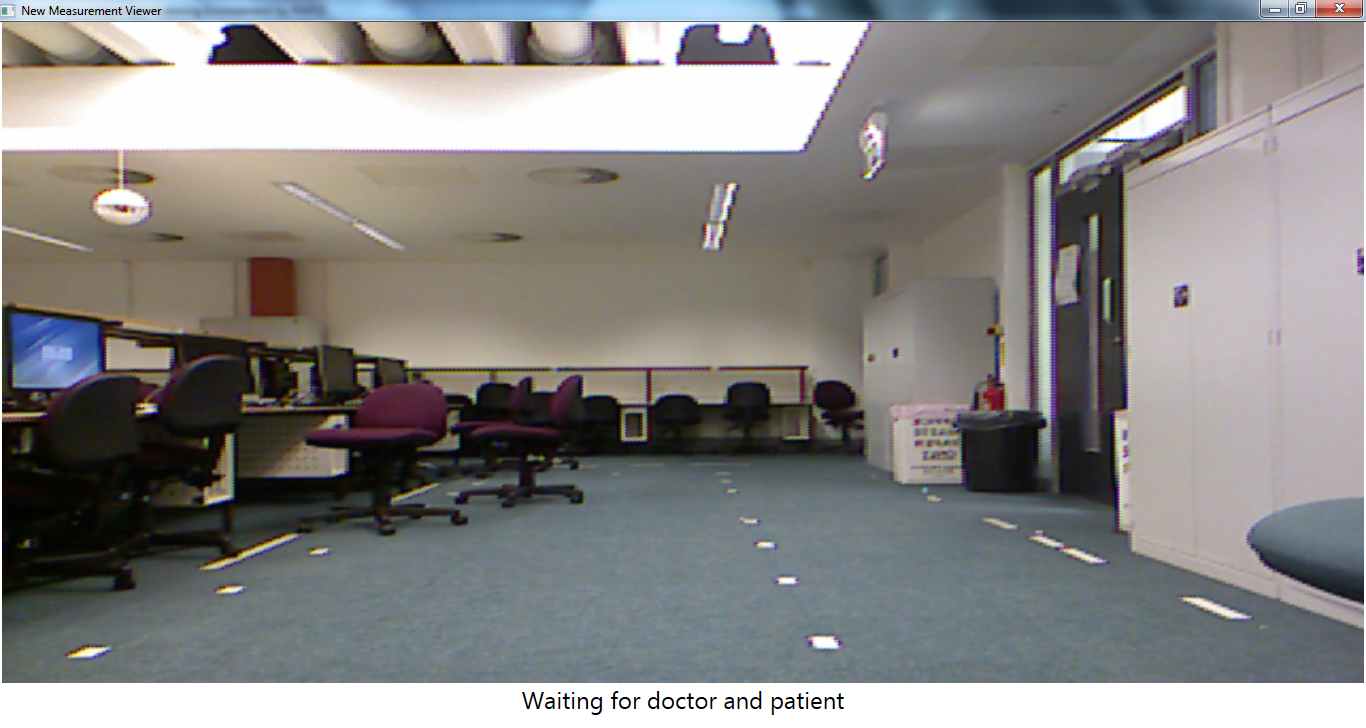
\includegraphics[scale=0.25]{zscreenshots/MeasurementLoader2.png}}\\
    \caption{MeasurementLoader: The large, clear display indicates the next step}
\end{center}

\section{Person Isolation}
\label{testing:person isolation}
This section details the testing of the depth based person isolation.\\

\subsection{Isolating Multiple Subjects}
During the design of depth based person isolation in Section \ref{imp:depth based isolation}, the isolation was determined to be sufficient for one person. Further testing was conducted on multiple subjects to confirm that the method would work on many people, rather than only the subject in Figure \ref{fig:depth and hand based cut off}. Figure \ref{fig:multiple subjects isolated} show the behaviour of the isolation method on the aforementioned multiple subjects. From this figure, the isolation method can be said to work consistently on many subjects.\\

\begin{figure}[h]
\begin{center}
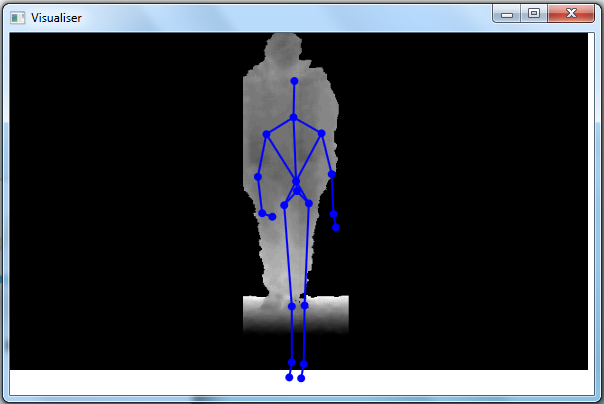
\includegraphics[scale=0.3]{images/bernie_iso} 
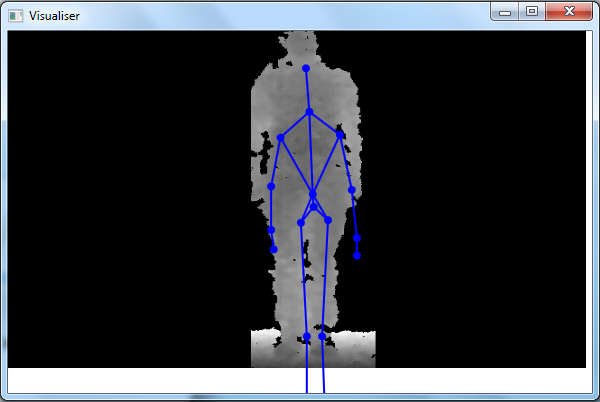
\includegraphics[scale=0.3]{images/page} 
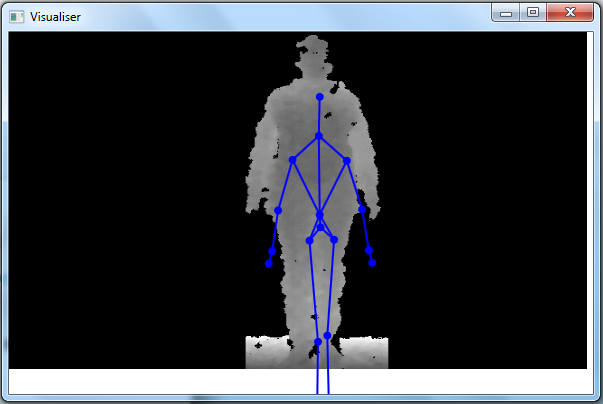
\includegraphics[scale=0.3]{images/steffat} 
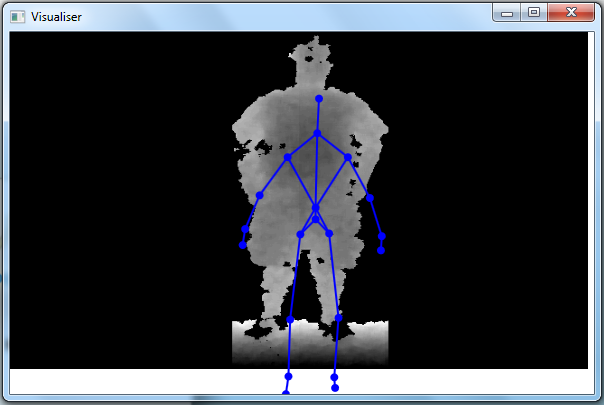
\includegraphics[scale=0.3]{images/wilkoiso} 
\end{center}
\caption{Multiple subjects isolated.}
\label{fig:multiple subjects isolated}
\end{figure} 

\subsection{Floor Removal}
As previous noted in Sections \ref{design:depth based isolation} and \ref{imp:depth based isolation}, the depth based cut off leaves the floor underneath the person as an unwanted artifact in the final point cloud. Fortunately, the floor can be removed at the point cloud level as suspected. An example of this action is shown in Figure \ref{fig:floor removal}.\\

\begin{figure}[h]
\begin{center}
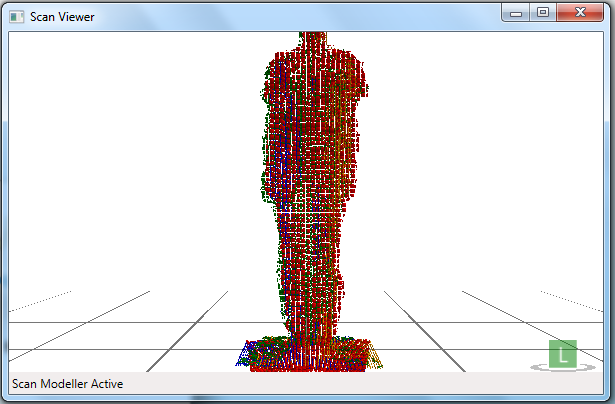
\includegraphics[scale=0.3]{images/greg_feet}
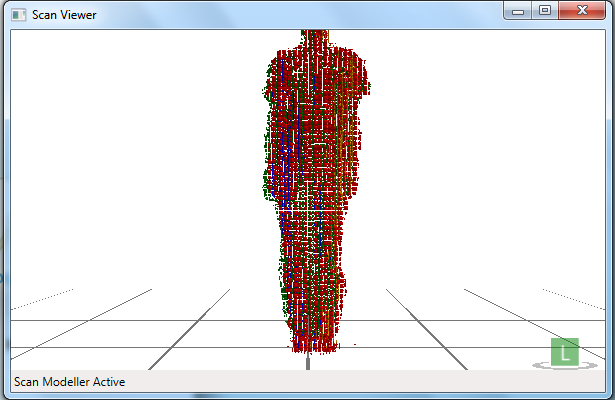
\includegraphics[scale=0.3]{images/greg_nofeet} 
\end{center}
\caption{Left: The point cloud with the floor. Right: After floor removal.}
\label{fig:floor removal}
\end{figure} 
\section{Point Clouds}
\label{impl:point clouds}
\subsection{Data Structure}
The K-D tree data structure, discussed in section was partially implemented by a third party open source library, which was then generalised to accommodate the point structures. \\

Additional C\# primitive data structures were utilised to maintain meta information about the point cloud such as maximum and minimum values; information about the resolution of the image from the input device and data about the input device. \\ 

\subsection{Conversion to real world coordinates}
The conversion from a depth map to the real-world coordinate system is as follows. The depth map is scanned, progressively incrementing $i_x$ and $i_y$. At every stage the calculations in \ref{eq:pc conv x}, \ref{eq:pc conv y} and \ref{eq:pc conv z} are performed and then inserted into a \texttt{PointRGB} data structure along with the \emph{red}, \emph{green} and \emph{blue} values. An explanation of the variables in the equations just mentioned can be found in Table \ref{fig:pc conv meaning}. \\

\begin{equation}
    z = depthValue * scale
    \label{eq:pc conv z}
\end{equation} \\
\begin{equation}
    x = (centre_x - i_x) * z * f_{xinv}
    \label{eq:pc conv x}
\end{equation} \\
\begin{equation}
    y = (centre_y - i_y) * z * f_{yinv}
    \label{eq:pc conv y}
\end{equation} \\

\begin{table}[h!]
    \centering
    \begin{tabular}{ |c | c | c |}
    \hline
        Variable   & Meaning                  & Value \\ \hline
        $centre_x$ & centre of depth map (x)  & $\frac{640}{2}$ * \\
        $centre_y$ & centre of depth map (y)  & $\frac{480}{2}$ * \\
        $scale$    & fiddle factor            & $0.001$ \\
        $f_{xinv}$ & fiddle factor            & $\frac{1}{476}$ \\
        $f_{yinv}$ & fiddle factor            & $\frac{1}{476}$ \\  
        \hline
    \end{tabular}
    \caption[The meaning behind variables used in the depth map to point cloud algorithm]{The meaning behind variables used in the depth map to point cloud algorithm. * denotes a value that is specific to the PARSE implementation} 
    \label{fig:pc conv meaning}
\end{table} \\

\subsection{Merging point clouds}
There is no trivial way to attach on point cloud to another due to the way in which the K-D tree is structured. It is therefore necessary to take the points from one point cloud and then add them to the second one-by-one. Sometimes there are collisions, a point is defined in exactly the same place in the point cloud - especially in the overlapping areas after a good registration has taken place. When this happens the second point is simply discarded. \\

\subsection{Transformation}
To aid the registration process a number of key transformation functions have been implemented which operate directly on the data stored within the point cloud data structures. \\

\subsubsection{Translation}
The translation method simply works by translating all data in the point cloud and then translating the maximum and minimum values in each coordinate. \\

\subsubsection{Rotation}
The rotation method is slightly more complicated as rotation in a 3-D space necessitates the usage of the complex plane. The rotation is achieved through the utilisation of a quaternion and a rotation matrix. \\

\subsection{Floor removal}
A problem that occurred during the registration process was the floor getting in the way. This can be mitigated by calling the \texttt{removeFloor} method. The method simply removes the lower plane in the point cloud. \\

\subsection{Visualisation}
The visualisation was implemented using the Windows Presentation Framework with Helix 3D as a helper library. Each depth point in the point cloud was modelled as a small cube so that they may be displayed in a pleasing manner. Examples of visualisations may be seen throughout this report but specifically in section \ref{imp:stitching}.

\section{Volume Estimation}
\label{design:volume estimation}
There are many techniques for estimating an arbitrary metric of a given 3-dimensional shape, including the volume of the shape.
Focus will first be on height estimation to see if the methods can be extended to calculate volume, before moving to methods specifically designed for volume estimation.\\

\subsection{Estimating the Height of Trees}
LIDAR has previously been used to estimate the height of trees from above \cite{Maltamo2006}. Three laser scanning-based methods were used to compute the height of the trees: a direct prediction model for the stem volume at plot level, a volume prediction system based on the modelled percentiles of the basal area diameter distribution and a parameter prediction method used to determinate Weibull based basal area diameter distributions \cite{Frechet1927} for the plot-level stem volume prediction. The best results were obtained with the first method, i.e. the model that predicts plot-level stem volumes directly \cite{Maltamo2006}.\\

In order to calculate the height, the laser reflections from non-ground objects, such as trees and buildings were classified as non-ground hits using TerraScan software \cite{Solid2013}. Conversely, other points were classified as ground hits. Canopy height of a non-ground object is then calculated as the difference between the height of the non-ground object and the neighbouring ground points. The accuracy of this method was found to be better than $\pm$15cm \cite{Maltamo2006}, when compare to field-measured volumes obtained with the Finnish conventional method Inventory by Compartments \cite{Koivuniemi2006}.\\

It should be noted that in this method the LIDAR emitter was above the target \cite{Maltamo2006}, rather than in front, as is likely in the case of this project. This method then translates to use the top and the bottom most point of the cloud to calculate height. However it may be extendable to calculate metrics such as depth and breath, from which a minimum bounding box could be determined.\\

A minimum bounding box is defined as follows in Figure \ref{fig:bounding_box_definition}.\\

\begin{figure}[h]
\textit{Definition: For a point set in N dimensions, it refers to the box with the smallest measure (area, volume, or hypervolume in higher dimensions) within which all the points lie} \cite{Barequet2001}.
\caption {Minimum bounding box definition}
\label{fig:bounding_box_definition}
\end{figure}\\

For the purposes of the project, the bounding box would be three dimensional and the volume of the minimum bounding box calculated as in equation \ref{eq:calculating_the_volume_of_the_minimum_bounding_box}.\\

\begin{equation}
    \label{eq:calculating_the_volume_of_the_minimum_bounding_box}
    Volume = (xmax -xmin) * (ymax - ymin) * (zmax - zmin)
\end{equation}\\

Such a box may be useful in calculating an upper bound on the volume of the patient.\\

\subsection{Determination of prostate volume by transrectal ultrasound}
The volumes of prostates have previously been calculated from ultrasound scans using many methods, including step-section planimetry and the elliptical volume method. After the volume of the prostate was estimated, all patients in the study underwent subsequent radical prostatectomy or cystoprostatectomy and prostate specimen weights were compared with the results of each volume estimation method \cite{K1991}.\\ 

\subsubsection{Step-Section Planimetry}
\label{research:ssp}
Step-Section Planimetry (SSP) is so called because of the planimeter, a measuring instrument used to determine the area of an arbitrary two-dimensional shape by traversing the perimeter \cite{Bryant2011}. 
The method calculates the area at each step, uses these areas to calculate the volume of a step and then sums these volume to determine the total volume. SSP is similar to the technique of volume rendering, which uses multiple two-dimensional slices to build up a three-dimensional image.\\

For simplicity's sake, let $O(p) \in O(p)$, where $p$ is the number of points in the point cloud.\\

The method traverses the point cloud representation of an object, requiring again at most $O(y)$ where y is the number of points in the y axis. Again for simplicity, let $O(y) \in O(p)$. Hence, the total SSP method will run in $O(p^2)$. Whilst the area/volume is being calculated, other useful metrics could be determined, such as the perimeters of the steps\footnote{or planes}.\\

Algorithmically, the area/volume could be calculated with the Shoelace formula \cite{Pretzsch2009}. The Shoelace formula states that, given a polygon made up of points $\{(x_1,y_1),(x_2,y_2)...(x_n,y_n)\}$ ordered clock-wise\footnote{or anti-clockwise}, the area can be calculated as in equation \ref{eq:the shoelace formula}. The Shoelace formula is the mathematical equivalent of a planimeter.\\

\begin{equation}
\label{eq:the shoelace formula}
Area = \left|\frac{(x_1y_2 - x_2y_1) + (x_2y_3 - x_3y_2) + ... + (x_ny_1 - x_1y_n)}{2}\right|
\end{equation}\\

Similar methods to SSP have been used in other areas of medicine, such as measuring brain, heart and fetal lung volumes \cite{Rosen1990,Rypens2001,Graham1971}.\\

\subsubsection{Elliptical volume}
Much like a bounding box, an ellipsoid can be formed around a person using their height, depth and breadth and the volume of this ellipsoid is then calculated using the formula in equation \ref{eq:calculating the volume of an ellipse}, where $a,b,c$ are the lengths of the axis.\\

\begin{equation}
Volume = \frac{4}{3}\pi abc
\label{eq:calculating the volume of an ellipse}
\end{equation}\\

For prostates, the elliptical volume method demonstrated a correlation coefficient of 0.90 \cite{K1991}. Again, this suggests a high accuracy. However, this high performance may be due to the roughly walnut shaped nature of a prostate \cite{D2003}. 
On a less spherical object, such as a person, the elliptical method may output a higher volume than the true value, as with the bounding box.\\

If the min and max values of a object were stored in it's point cloud, the ellipsoid could be computed in $O(1)$, similar to the bounding box. 
If the min and max values need to be computed on the fly, this would bring the complexity up to $O(p)$, putting the ellipsoid method's complexity less than the step-section method. As elliptical volume is less accurate and cannot give other information, such as perimeter, step-section will be the basis of volume calculation design.\\

\subsubsection{Convex Hulls}
Because the Kinect depth data has high level of noise, it may be necessary to compute the convex hull of a plane in order to obtain more accurate results. Three convex hull methods were researched, Gift-Wrapping \cite{Cormen2001}, Quick Hull \cite{Barber1996} and the Kirkpatrick--–Seidel algorithm \cite{kirkpatrick1986}.\\

Gift-Wrapping (GW), also known as Jarvis' march \cite{Jarvis1973}, is similar in two dimensions to the process of winding a string around the set of points. 
GW runs in $O(nh)$ \cite{Cormen2001} where $n$ is the number of points in the input and $h$ is the number of points in the hull. In the case of this project, it is likely that $O(h) \in O(n)$ as the points are expected to already be almost hull like. 
Hence GW can be, for the purposes of the project, said to run in $O(n^2)$. However, GW is simple to implement so may be the method chosen by the group.\\

Quick Hull (QH) uses a divide and conquer approach similar to that of QuickSort, which it's name derives from. Its average case complexity is considered to be $O(n * log(n))$, whereas in the worst case it takes $O(n^2)$ \cite{Barber1996}. As previously stated, project data is likely to be near to the worst case. Hence, QH may perform no better than GW and may be more difficult to implement. The convex hull is unique for a given point set \cite{Sedgewick2012}, so accuracy is not a concern when picking an algorithm.\\

The Kirkpatrick--–Seidel algorithm runs strictly in $O(n*log(h))$, for the purposes of the project, this becomes $O(n*log(n))$. Whilst KS has a lower complexity than GW, it may be more time-consuming to implement. As such, the group may opt for GW if a convex hull algorithm is indeed needed.\\
\section{Limb Circumference}
\label{design:limbcircum}

The design of algorithms used for calculating limb circumference builds on the design principles of planimetry and as identified in section 3.6.1, this forms a reasonable basis for calculating circumferences using range imaging. 

\subsection{Plane Partitioning}

The limb circumference approach uses the sames SSP methodology for the estimation of volumes, pulling out planes using the shoelace formula. Hence limb circumference will operate on the same basis of the full body scan. Due consideration was given to alternative scanning contexts, where localised scanning would take place around a particular limb. However, as per the functional requirements of the system, we wanted to minimise the amount of configuration and patient setup required for the capturing of these measurements. The resolution of the Kinect device for capturing and tracking limb circumference, with it's 11-bit depth and 2048 levels of sensitivity was deemed adequate for estimating these metrics at distance. \\

Plane partitioning is achieved by using a mapping between the skeletal feature points and the point cloud isolated from the depth map. The 20 skeletal feature points are defined in terms of \emph{real-world coordinates} inferred from the depth map representation. The $(x,y,z)$ co-ordinates of these feature points are related by the inferred body part identification. With this, a bounding box around the limb is first determined in real-world coordinates. These bounds are defined by taking the minimal and maximal x,y coordinate's from the feature points for the limb. These bounds are then transformed into the point cloud co-ordinate system. The relative depth of the limb skeletal feature points are identical to the depth of the point cloud and as such do not require this transformation. \\

\begin{figure}[ht]
\begin{center}
$PC_n_e_w(x,y) = ((C_x,C_y) - (x,y)) * zz * f_x_,_yinv$
\end{center}
\caption{Translation from Real-world to Point Cloud co-ordinate system}
\label{fig:conversionformula}
\end{figure}

$C_x$ and $C_y$ are defined as the centre of the captured depth map of resolution 640x480 pixels. The depth map is then scaled by a constant $zz$ defining the size of the points that will be used to represent the point cloud in the 3D visualisation. The point is then multiplied by the invariants $f_x_,_yinv$. The importance of using this arbitrary point cloud space is highlighted by the unique set of points it generates that can then be represented accurately. It also allows information defined in real-world coordinates such as a the aforementioned skeletal data to be associated with each captured point cloud.

\subsection{Circumference Calculation}

The algorithm then subsamples on the n returned planes from the partitioned point cloud but uses the planes equidistant between the limb joints to give a mean representation of limb circumference on the selected limb. The circumference of each plane is calculated using the \emph{Gift Wrapping} algorithm, as detailed in the research section of the report, which returns the convex hull of a set of points. In the case of the PARSE implementation, we pass a subsampled region of planes and for each y return a convex hull which is then averaged for the mid-region for the particular limb. Similar to the estimation of Volume, the circumference returned is not defined in terms of SI units but rather determined in terms of the point cloud. This will require further testing to ascertain a suitable multiplicative constant to obtain a reasonable approximation to the circumference of the subject. \\

\subsection{Algorithm Running Time}

This algorithm enumerates each limb and performs plane partitioning and circumference calculation in real time. Because the algorithm itself is derived from the volume calculation and planimetry used to calculate whole-body volume, it is sensible to assume a similar running complexity to $O(\sqrt[3]{p}^2)$. The running complexity of calculating limb circumference is further compounded by the limb enumeration and bounding box calculation step where $O(n)$ represents the possible number of times the planimetry algorithm is to be run and $O(n^2)$ for each bound for those limbs to be calculated.

\subsection{Alternative Approaches}

Apart from the direct partitioning of this abstract point cloud structure and the calculation of the convex hull for each of the extracted planes, there are other means of limb circumference measurement that uses least squares regression for the fitting of ellipses to scatted 3 dimensional data, something that could be easily extended to calculation of circumference for a given point cloud region based on the fitted ellipses. Fitzgibbon et al. \cite{Fitzgibbon1999} fit these primitive ellipses to provided image data by finding the set of parameters that minimise the distance between the provided data points and the proposed ellipse shape.  While this least squares method is only used on scattered data in 2 dimensional space, this method could be viably extended into 3D space as has been achieved by Geiger who proposes a method which registers the persons point cloud in different poses and projects the captured 3 dimensional data into 2D space for registering the circumference as the person rotates \cite{Geiger2011}.



%complete
\section{Point Cloud Stitching}
\label{design:registration}
\label{design:sitching} %legacy, do not remove
\label{design:stitching}
The specification states that only a single scanner is to be used. This necessitates the utilisation of multiple scans and the stitching thereof into one unified data structure. This data structure can then be manipulated to produce volume estimation, as described in Section \ref{design:volume estimation}. The process of stitching these point clouds together to create one unified dataset is known as \emph{registration}\cite{Makadia2006} which has been described in Section \ref{research:registration}. The development of ideas leading to the final algorithm will be described in this section.  \\

\subsection{Input Data}
Depth maps of people (shells) are to be passed to the registration algorithm from a \emph{person isolation} subsystem. 

\subsection{Design Pattern}
\label{design:design pattern}
The various point cloud stitching algorithms all extend a class called ``Stitcher``. This makes it easy for new stitching algorithms to be deployed within the PARSE environment as only a single line of code needs to be modified in order to use a different stitching algorithm.\\

\subsection{Initial Experimentation}
Initially the point clouds were stitched by rotating successive scans 90\degree \ , increasing by a further 90\degree \ for each previous scan that has been taken, in an anticlockwise direction. The scan was then translated by a constant vector to produce a reasonable point cloud. This was able to produce reasonable results in individual cases but people come in a variety of ``depths`` and such an algorithm would only be useful in a world where everyone had constant "depths". \\

\subsection{Development of a more sophisticated approach: Bounding Boxes} 
\label{design:bounding boxes}
\label{design:bounding box}
While the Kinect is designed to produce depth information, it is only capable of scanning the visible surfaces of objects in front of the point in the 3D world in which it is situated. This has led to the coining of the term \emph{2.5D} to explain the limited information that the Kinect, and all single depth sensors, are able to gain about the world around them \cite{lu2006}. In theory this very limitation can be exploited to produce a reasonable, but by no means perfect, point cloud registration most cases. Within the context of this project this has come to be known as the \emph{Bounding Box} method of point cloud registration. \\ 

\subsubsection{Scanning Phase}
As with the initial experimentation, the bounding box method requires four scans; $S_1, S_2, S_3, S_4$. After each scan is obtained the patient is rotated by 90\degree \ in an anti clockwise direction. Each scan contains length and width information which is used in the processing phase. These scans are then packaged into a list data structure and sent to the bounding box method for processing. \\

\subsubsection{Processing Phase}
The processing phase consists of a number of simple rotations and translations. The subject was only rotated about the vector $(0, 1, 0)$ which significantly reduced the complexity of the operations. Table \ref{tab:bb processing} shows the rotations and translations that were performed for each scan. \\

%table 
\begin{table}
    \begin{tabular}{| p{0.8cm}| p{1.4cm} | p{4.9cm} | p{3.9cm} |}
    \hline
        Scan & Rotation & Rotation Axis & Translation  \\
        \hline
        $S_1$ & 0 \degree & $(0, 0, 0)$ & (0,0,0)  \\
        $S_2$ & 90 \degree & $(S_2(x_{min}), S_2(y_{min}), S_2(z_{min}))$ & $(0, 0, width)$  \\
        $S_3$ & 180 \degree & $(S_3(x_{min}), S_3(y_{min}), S_3(z_{min}))$ & $(S_3(width), 0, S_2(width))$  \\
        $S_4$ & 270 \degree & $(S_4(x_{min}), S_4(y_{min}), S_4(z_{min}))$ & $(S_3(width), 0, 0)$  \\
        \hline
    \end{tabular}   
    \caption{The processing that takes place on each data item for the Bounding Box method}
    \label{tab:bb processing}
\end{table} \\

\subsubsection{Challenges}
Despite the apparent successful stitching in many cases, the \emph{Bounding Box} method produced erratic results occasionally. Due to anatomical differences, male subjects tended tended to be stitched more accurately than female ones. This was also the case with obese subjects. This problem has been internally known as the \emph{Breast Problem} (Section \ref{testing:the breast problem}). \\

To address this; a more sophisticated registration method, the Iterative Cloud Positioning (ICP) algorithm (Discussed in Section \ref{res:icp}) was investigated. One of the big problems with the ICP algorithm, and other registration algorithms, is that they require some form of initial alignment which is then improved over time. This initial problem had already been potentially solved using the Bounding Box method and so it has been utilised part of a processing pipeline. \\

\subsection{Manual Alignment}
As discussed in the previous section, it is necessary that some form of initial alignment is made before most algorithms would be useful. To address the breast problem (Section \ref{testing:the breast problem}) it could be possible to offer some kind of manual alignment of the body panels. This, however, would potentially introduce unpredictable human error and would require real-time visualisation and modification of the point cloud data structures. Performing just four rotations and one rendering, as in the Bounding Box method \ref{design:bounding box}, takes several seconds to complete and therefore a new trade-off of image resolution vs display and processing hardware would be introduced. The manual alignment idea was ultimately abandoned due to the overriding objective of keeping the final product cheap in terms of hardware requirements, accurate and easy for the operator to use. \\

\begin{figure}[h!!]
    \label{fig:registration pipeline}
    \begin{center}
        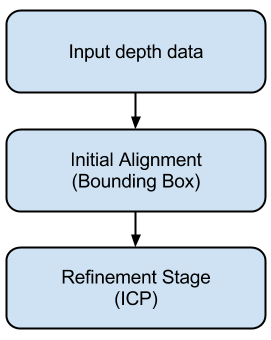
\includegraphics[scale=0.6]{zscreenshots/reg-pipeline.png}
        \caption{A pipelined approach towards registration}
    \end{center}
\end{figure}

\subsection{Final design: Iterative Closest Point (ICP) algorithm}
So far it has been explained how a simple method that is the bounding box method is able to produce reasonably good results. In Section \ref{res:icp} we learnt that the gold standard for registration is the Iterative Closest Point method which requires some initial alignment. This alignment could be provided by the bounding box method. \\ 

Using the information that from experimentation and the research in Section \ref{res:icp} a pipelined approach to registration was developed using the three steps, explained in Figure \ref{fig:registration pipeline}.


\section{Markerless Recognition}
The markerless recognition problem was approached in two phases. First, the sensor's location was to be tracked using the video image feed from the Kinect. Then, this location would be translated into 3D space using information from the depth feed, and finally the sensor's position relative to the body could be calculated. This mechanism could then be used either just once, to register a new position, or on every frame, to guide the sensor to a target position.\\

Three different algorithms were tested for effectiveness in the application: one robust algorithm - SURF, a non-robust algorithm - Haar classification, and a simple colour search.\\

\subsection{Colour Search}
The colour search tests intend to answer three questions:
\begin{enumerate}
\item How effective is searching for a specific colour?
\item How much difference is there between searching the RGB and HSL colour spaces?
\item What is a ‘good’ colour to search for?
\end{enumerate}

In order to answer these questions, the colour searching mechanism must allow for ranges of colours to be searched for, and in either of the RGB or HSL colour spaces. \\

For testing, a separate application was designed, which would analyse the video feed from the Kinect. A simple check highlighted values in the output image on a binary basis: matches in white, the rest in black. A more efficient algorithm, if needed, would be put in place during any further development.\\

\subsection{Haar}
Early in the project, Haar classifiers were considered to be a viable option. Highly rated by users of the imaging library PCL, in use by the project at that time, the Haar classifier appeared worthy of testing. The premise was that, once trained on sufficient data, a Haar classifier could be applied to imagery in real time, thus giving a highly responsive tracking system.\\

The PCL imaging library provides numerous algorithms written in C, available within a C# wrapper. This gives the user the potential to create a highly efficient program. Such usage does however expose the library’s C heritage with the requirement in many places to pass in memory allocations and pointers, which is a drawback for some. \\

The initial design plan was to first learn the classifier generation procedure, and then run basic tests on its effectiveness. If sufficiently reliable, a system would then be devised which could use a collection of classifiers in parallel. One of the drawbacks of Haar classifiers is their sensitivity to rotational variance. This is acceptable in many situations, for example face detection in photographs, but would not be helpful in the defined situation of this project. Thus, a system would be devised and tested, which would utilise a collection of classifiers generated for the target at different rotations.\\

\subsection{SURF}
The OpenCV library provides an implementation of the SURF algorithm, and this was used to create a classifier suitable for testing. This, combined with SURF's reputation for high speed, led to it's use over SIFT. In reality, however, it was not possible to run this SURF implementation in real time. Each SURF run took a few seconds, which made video or real-time testing impossible. The SURF classifier was therefore tested only on static images. \\

The default parameters were investigated, and the setup was deemed sufficient for the tests.\\

The program was configured to output a single image containing, on the right side, the target image with its features highlighted, and on the left side the input image with its features highlighted. Any correspondences between the two images’ features are indicated with lines, and any target identified is indicated by a rectangle.\\

\subsection{Scan Process}
The method for taking a tracked scan needed to be as simple as possible, and make intuitive actions where possible. One such measure is to allow automatic triggering of the capture event when the scanner is held still. This should mean that, once started, no further interaction with the computer is necessary to complete the scan process - an important time-saving feature, should the operator be working alone.\\

Once initiated, the scan process will immediately begin searching for and tracking the target sensing device, the operator and the patient. After determining the operator and the patient, the program will wait for the sensing device to be held still for a number of seconds before automatically triggering the capture routine, and closing the window.\\

\section{External Libraries}
A number of external libraries have been used to provide data abstraction and optimised functionality. This section will explore details about their licensing and usage within the PARSE toolkit. \\

\subsection{Kinect SDK}
The Kinect SDK was the basis for the development of the project but the group only utilised a subset of it's functionality as our specialist point cloud reconstruction and volume estimation required access to the raw depth feed as necessitated for reconstructing the body. The SDK itself provided a means of accessing functions which allowed data to be mapped onto different coordinate spaces for the reconstruction of the point cloud. The Skeletal tracking technology also provided by the Kinect was used extensively in order to when a body is in view of the kinect for calibration, scanning, and markerless recognition purposes. It has also been used for the basis of isolation as it provided useful cues as to the appropriate level at which to perform a depth cut off. \\ 

\subsection{Math.NET}
A library called Math.NET was utilised extensively in the ICP portion of the solution to make up for the lack of support for data structures representing matrices and their associated operations within C# and the .NET framework \cite{mathdotnet}. The framework only contained basic operations such as additive and multiplicative operations and contained only a small subset of the operations that are available in an application such as MatLAB. Due to the lack of free matrix manipulation libraries Math.NET was used as a compromise and much of the matrix manipulation functionality was re-implemented in a specialised manner for this project. It is available under the MIT/X11 license which is a permissive licence allowing the usage of the software in both free and commercial applications as long as attribution is given \footnote{Fulltext available at: http://www.xfree86.org/3.3.6/COPYRIGHT2.html}. \\

\subsection{Helix3D}
Helix3D is a WPF based visualisation framework which adds a number of helper functions and viewport interactivity to the existing WPF3D framework \footnote{HelixLink}. Since it's inception, WPF3D has generally been considered a poor alternative to more established high performance frameworks such as OpenGL \cite{WpfPoor} but due to our language choice and the declining support of DirectX, WPF3D combined with Helix provided an adequate means of visualising the reconstructed point clouds and planes extracted from segmented point clouds after volume calculation and limb circumference determination. \\  

\subsection{WpfToolkit}
\label{design:wpf}

WpfToolkit added further functionality to the Windows Presentation Framework such as charting and visualisation for Markerless recognition/recall tasks. \\
\section{Interface Design}
\label{design:interface}

The interface was designed using the WPF framework. Each component of the user interface was written to support it's respective functionality and each UI unit is self contained. The use of a centralised class for dispatching events and handling core functionality means that data present in each functional UI unit of the system can be accessed via the relevant procedures in the CoreLoader. This allows the respective functions access to each others data and methods where appropriate.

\subsection{Intended Audience}

It is anticipated that this project will be used by researchers or medical practitioners on a initial patient examination level rather than on a diagnostic basis. Therefore the functionality of the system and the results it returns need to presented in a way which can be easily understood by both medical practitioners and the general public. This is as per the non-functional requirements facilitated through an adequate user interface.

\subsection{Component Design}

For the design of each component of the UI, the group agreed to follow the MVVM design pattern where the business and presentation logic of the system is separated from the technicalities of implementing the user interface. This meant that we could use the user interface to expose the data objects generated by visualisations or calculation of volumes or circumferences. WPF does not actually support the MVVM pattern of design due to all user interface components using an underlying XAML representation with access to data objects permitted by a data binding at run time. This required us designing the interface that would emulate such functionality. This was achieved by using separate user controls that would bind to each data object generated by the functionalities of the system.

Each user interface component uses a \texttt{\_Loader} convention to signify it's relation to the CoreLoader interface. The CoreLoader UI component is the parent class of all other UI components. This means child components can consist of other windows or custom user controls. It also reflects the architecture of the system. 

\subsubsection{CoreLoader}

This component is the owner of all other user interface components. This means that any global operations applied to this component affect all other currently open components. CoreLoader provides access to all the functions of the system.

\subsubsection{ScanLoader}

ScanLoader contains the viewer for visualising models representative of scanned pointclouds. ScanLoader allows for interaction with the model including panning and zoom as well as permitting aesthetic changes to the model such as colour or rendering.

\subsubsection{ViewLoader}

This component shows the raw data and overlay streams of the Kinect device. ViewLoader is capable of representing colour, depth and skeletal as well as feeds that incorporate additional post processing such as depth isolation or color isolation of a given subject.

\subsubsection{HistoryLoader}

HistoryLoader shows the results of any volume or limb circumference calculations carried out on a patient. These calculations will also be visualised depending on if planes need to be visualised for volumes. HistoryLoader also contains charting of results according to previous scans that the patient may have been subjected to in order to show changes in measurement for both limb circumference and volume.

\subsubsection{PatientLoader}

PatientLoader is a component that allows for the entry, editing and viewing of details related to the patient that is stored on the system database. 



\newpage
\section{Summary}
This section summarises the above design decisions.\\

\subsubsection{Person Isolation}
The depth and colour based isolation, described in \ref{design:depth based isolation} based on Kinect skeleton data was used over KDE and MOG. This route was taken because similar computation complexity of depth based isolation, the capability to isolate stationary people and the ease of implementation.\\

\subsubsection{Registration}
Point clouds will be stitched together using the Iterative Closest Point algorithm due to its proven good quality results over the past decades. This has been explained further in Section \ref{research:registration}. Initial alignment will assist the ICP algorithm using the bounding box methodology. These two steps should produce a point cloud that can be used by the calculations explained in this section to a satisfactory degree of accuracy. \\

\subsubsection{Volume Estimation}
The volume estimation continues to build on the SSP methodologies originally researched. The algorithm will split the point cloud into planes and calculate the area of each, using the Shoelace formula. Each area will then be multiplied by the distance between the planes to give a volume. These volumes will then be summed to give the final output. Not only is the volume calculated, but the circumference of each plane used has been calculated to provide additional information.\\

\subsubsection{Markerless Recognition}
Testing will reveal the effectiveness of three image search methodologies, RGB colour space search, SURF, and Haar-based classification. The most effective will be used as the basis for the scanner tracking. From there, translation to the real coordinate space and use of the Kinect's skeleton tracking API should allow the calculation of skeleton-relative positions.
